\documentclass{standalone}
\usepackage{tikz}
\RequirePackage{palatino,mathpazo}
\RequirePackage[scaled=1.02]{inconsolata}
\RequirePackage[T1]{fontenc}
\begin{document}
% This code uses the tikz package
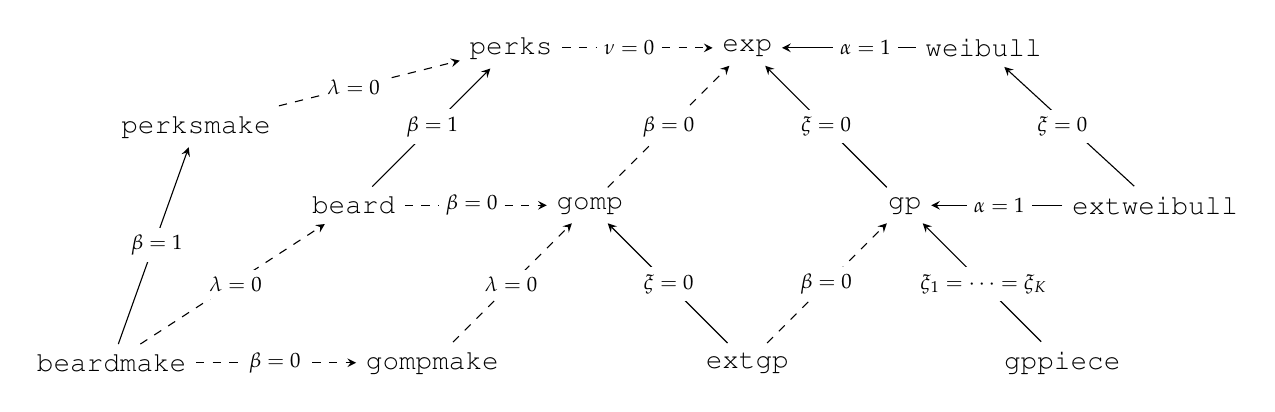
\begin{tikzpicture}[scale=2]
\node (v0) at (0.00,0.00) {\texttt{exp}};
\node (v1) at (-1.00,-1.00) {\texttt{gomp}};
\node (v2) at (1.50,0.00) {\texttt{weibull}};
\node (v3) at (1.00,-1.00) {\texttt{gp}};
\node (v4) at (0.00,-2.00) {\texttt{extgp}};
\node (v5) at (-2.00,-2.00) {\texttt{gompmake}};
\node (v6) at (2,-2.00) {\texttt{gppiece}};
\node(v7) at (-1.5, 0) {\texttt{perks}};
\node(v8) at (-3.5, -0.5) {\texttt{perksmake}};
\node(v9) at (-2.5, -1) {\texttt{beard}};
\node[left](v10) at (-3.5, -2) {\texttt{beardmake}};
\node [right](v11) at (2.0,-1) {\texttt{extweibull}};
\draw [-stealth, dashed] (v1) edge (v0);
\draw [-stealth] (v2) edge (v0);
\draw [-stealth] (v3) edge (v0);
\draw [-stealth, dashed] (v8) edge (v7);
\draw [-stealth, dashed] (v10) edge (v9);
\draw [-stealth, dashed] (v10) edge (v5);
\draw [-stealth, dashed] (v9) edge (v1);
\draw [-stealth, dashed] (v7) edge (v0);
\draw [-stealth] (v10) edge (v8);
\draw [-stealth] (v9) edge (v7);
\draw [-stealth] (v4) edge (v1);
\draw [-stealth] (v11) edge (v2);
\draw [-stealth] (v11) edge (v3);
\draw [-stealth, dashed] (v5) edge (v1);
\draw [-stealth, dashed] (v4) edge (v3);
\draw [-stealth] (v6) edge (v3);
\node[scale=0.75,fill=white] at (-0.5,-0.5) {$\beta=0$}; %Gomp vs exp
\node[scale=0.75,fill=white] at (-0.75,0) {$\nu=0$}; %Perk vs exp
\node[scale=0.75,fill=white] at (-2,-0.5) {$\beta=1$}; %beard vs perks
\node[scale=0.75,fill=white] at (-3.75,-1.25) {$\beta=1$};
\node[scale=0.75,fill=white] at (-3.25,-1.5) {$\lambda=0$};
\node[scale=0.75,fill=white] at (-1.75,-1) {$\beta=0$};
\node[scale=0.75,fill=white] at (0.75,0) {$\alpha=1$};
\node[scale=0.75,fill=white] at (1.6,-1) {$\alpha=1$};
\node[scale=0.75,fill=white] at (0.5,-0.5) {$\xi=0$};
\node[scale=0.75,fill=white] at (2,-0.5) {$\xi=0$};
\node[scale=0.75,fill=white] at (-1.5,-1.5) {$\lambda=0$};
\node[scale=0.75,fill=white] at (-3,-2) {$\beta=0$};
\node[scale=0.75,fill=white] at (-2.5,-0.25) {$\lambda=0$};
\node[scale=0.75,fill=white] at (1.5,-1.5) {$\xi_1=\cdots =\xi_K$};
\node[scale=0.75,fill=white] at (-0.5,-1.5) {$\xi=0$};
\node[scale=0.75,fill=white] at (0.5,-1.5) {$\beta=0$};
\end{tikzpicture}
\end{document}
dag <- dagitty::dagitty('dag {
A [pos="0.000,0.000",label="exp"]
B [pos="-1.000,1.000",label="gomp"]
C [pos="1.000,0.000",label="weibull"]
D [pos="1.000,1.000",label="gp"]
E [pos="0.000,2.000",label="extgp"]
F [pos="-2.000,2.000",label="gompmake"]
G [pos="2.000,2.000",label="gppiece"]
H[pos="1.000,1.000",label="extweibull"]
A -> B
A -> C
A -> D
B -> E
B -> F
D -> E
D -> G
C -> H
G -> H
}'
)
plot(dag)
